\documentclass[12pt]{article}
\usepackage{hyperref}
\usepackage{amsmath}
\usepackage{amsfonts}
\usepackage{amssymb}
\usepackage{graphicx}
\usepackage{caption}

\title{\Huge\textbf{CS215 Assignment 1}}
\author{\Large\textbf{ Group Members :} \\ \\ 
    \large B.Abhinav  23B1018 \\ \\ 
    \large G.Abhiram  23B1084 \\ \\
    \large Sai Likhith 23B1058 
} 
\date{\today}

\begin{document}
\pagenumbering{arabic}
\maketitle
\newpage

\tableofcontents
\newpage

%%%%%%% QUESTION 1 %%%%%%%%%%%%%%
\section{Let’s Gamble}

There are two friends playing a dice-roll game. Friend A has (n + 1) fair dice and Friend B has n
fair dice (a fair die has equal probability of every face). On every roll, a win is achieved if we get a
prime number on the top. What is the probability that A will have more wins than B if both roll
all of their dice?\\
\newline
\textbf{Answer: 1/2}
\newline \newline
\textbf{Solution: }
\newline
A has (n+1) fair dice and B has n fair dice. The probability that a prime number comes on top in a single throw of a fair dice is $\left(\frac{3}{6}\right)\ =\ \left(\frac{1}{2}\right)$
as we have 3 prime numbers 2, 3, 5.
\newline \newline
Probability that A has i wins is equal to $\binom{n+1}{i}*\left(\frac{1}{2}\right)^{n+1}\ =\ \frac{\binom{n+1}{i}}{2^{n+1}} $.
\newline
Similarly Probability that B has j wins is equal to $ \frac{\binom{n}{j}}{2^{n}} $
\newline
We need to compute \newline $$\sum_{i=1}^{i=n+1}\sum_{j=0}^{j=i-1}\frac{\binom{n+1}{i}*\binom{n}{j}}{2^{2n+1}} $$ .
\newline
Let us compute the numerator.
\begin{equation}
    \sum_{i=1}^{i=n+1}\sum_{j=0}^{j=i-1}\binom{n+1}{i}*\binom{n}{j}
\end{equation}
Note that $\binom{n+1}{i} = \binom{n}{i} + \binom{n}{i-1} $ . Simplifies to:
\begin{equation}
    \sum_{i=1}^{i=n}\sum_{j=0}^{j=i-1}\binom{n}{i}*\binom{n}{j} + \sum_{i=1}^{i=n+1}\sum_{j=0}^{j=i-1}\binom{n}{i-1}*\binom{n}{j} .
\end{equation}

Using 
\begin{equation*}
\left(\sum_{k=0}^n \binom{n}{k}\right)^2 = 2^{2n}
\end{equation*}
    
\begin{equation*}
\sum_{k=0}^n \binom{n}{k}^2 = \binom{2n}{n}
\end{equation*}

We get the first term:
\begin{equation}
    \sum_{i=1}^{i=n}\sum_{j=0}^{j=i-1}\binom{n}{i}*\binom{n}{j} = \frac{2^{2n}-\binom{2n}{n}}{2}
\end{equation}

The second term on seperation turns out to be:
\begin{equation}
    \sum_{t=0}^{t=n}\sum_{j=0}^{j=t}\binom{n}{t}*\binom{n}{j} = \sum_{t=1}^{t=n}\sum_{j=0}^{j=t-1}\binom{n}{t}*\binom{n}{j} + \sum_{t=0}^n \binom{n}{t}^2  
\end{equation}

Use 2 and 3 it simplifies to:
\begin{equation}
    \frac{2^{2n}-\binom{2n}{n}}{2} + \binom{2n}{n} 
\end{equation}

Adding 3 and 5 to get the final value:
\begin{equation}
    2^{2n} - \binom{2n}{n} + \binom{2n}{n} = 2^{2n} 
\end{equation}

The final probability turns out to be :
\begin{equation}
    \frac{2^{2n}}{2^{2n+1}} = \frac{1}{2}
\end{equation}

\newpage
\section{Two Trading Teams}
You are playing a trading game against two teams A and B (will happen in reality soon). The
game is played in the form of a three-set series with A and B alternately. Also, Team B is better at
trading than Team A. To encourage your trading career, the exchange (an organization responsible
for managing the trades) gives you two options A-B-A (which means you play a game with Team A, then Team B and at last Team A again) or B-A-B. You will win if you win two sets in a row.
Which of the two options should you choose? Justify your choice with proper calculations.
\newline
\textbf{Solution: Choose B-A-B}
\newline \newline
\textbf{Solution: }
\newline
Assume the probability of winning against Team A is a and against Team B is b.\\
As Team B is better we have:  
\begin{equation}
    a > b
\end{equation}
Let us calculate the probability of winning for both cases.\\
\newline
\textbf{Case 1 : A-B-A} \\
For a win there are 3 scenarios : \textbf{W W W or W W L or L W W} . \\
Note that all three games are independent and hence we can multiply \\individual probabilities.\\
P(\textbf{W W W}) = aba , P(\textbf{W W L}) = ab(1-a) and P(\textbf{L W W}) = (1-a)bb .
The net probability is the sum of these 3 as they are exclusive: 
\begin{equation}
    P1 = aba+ab(1-a)+(1-a)bb = 2ab - a^2b = ab(2-a) 
\end{equation}
\newline
\textbf{Case 2 : B-A-B} \\
Just reverse a and b in the previous answer for probability here as both are similar.
\begin{equation}
    P2 = ab(2-b)
\end{equation}

Now we have $a>b$ hence $2-a<2-b$ which implies $ab(2-a)<ab(2-b)$ as $a,b$ are positive.
Hence 
\begin{equation*}
    P1\ <\ P2
\end{equation*}
\newline
\textbf{B-A-B is a better choice.}

\newpage
\section{Random Variables}
\begin{enumerate} \item Let $Q_1, Q_2$ be non-negative random variables. Let $\mathbb{P}(Q_1 < q_1) \geq 1-p_1$ and $\mathbb{P}(Q_2 < q_2) \geq 1-p_2$, where $q_1, q_2$ are non-negative. Then show that $\mathbb{P}(Q_1Q_2 < q_1q_2) \geq 1 - (p_1 + p_2)$ [3 marks]

    \item Given $n$ distinct values $\{x_i\}_{i=1}^n$ with mean $\mu$ and standard deviation $\sigma$, prove that for all $i$, we have $|x_i - \mu| \leq \sigma\sqrt{n - 1}$. How does this inequality compare with Chebyshev's inequality as $n$ increases? (give an informal answer) \end{enumerate}

\textbf{Solution: } 
\newline
\textbf{3.1: } 
From both the equations we can see that :
\begin{equation*}
    1-p_1 \leq P(Q_1<q_1) \leq 1\ \ and\ \    
    1-p_2 \leq P(Q_2<q_2) \leq 1  
\end{equation*}
Therefore
\begin{equation}
    p_1\geq0\ \ \ and\ \  p_2\geq0
\end{equation}
Let Event E1 be when $Q1<q1\ and\ Q2<q2$ . \\
Let Event E2 be when $Q1Q2<q1q2$ . \\
\newline
It is clear that E1 will imply E2 as $Q1<q1\ and\ Q2<q2$ always proves through multiplication $Q1Q2<q1q2$. \\
We can do this as they are non negative.
Hence $E_1 \subseteq E_2$ which implies $P(E_1) \leq P(E_2)$.\\
As $Q_1>q_1$ and $Q_2>q_2$ are independent we can multiply their probability to get the joint probability.
\begin{equation*}
    P(Q_1Q_2<q_1q_2) \geq P(Q_1<q_1)P(Q_2<q_2) \geq (1-p_1)(1-p_2) 
\end{equation*}
\begin{equation*} 
    P(Q_1Q_2<q_1q_2) \geq 1-p_1-p_2+p_1p_2 \geq 1-p_1-p_2\ as\ p_1,p_2 \geq 0
\end{equation*}
Hence we proved that:
\begin{equation*}
    P(Q_1Q_2<q_1q_2) \geq 1-(p_1+p_2)
\end{equation*}
\textbf{3.2: } If $\mu$ and $\sigma$ are the mean and standard deviation of the sequence, from definition of standard deviation we have:
\begin{equation}
    (n-1){\sigma}^2\ =\ \sum_{i=1}^{n}(x_i-\mu)^2   
\end{equation} 
As all terms of the summation are non negative we have
\begin{equation}
    \sum_{i=1}^{n}(x_i-\mu)^2\ \geq \ (x_i-\mu)^2 
\end{equation}
\begin{equation*}
    (x_i-\mu)^2\ \leq\ (n-1){\sigma}^2
\end{equation*}
Hence we proved that:
\begin{equation}
    |x_i-\mu|\ \leq \ \sigma\sqrt{n-1}
\end{equation}
\\
Now the Chebyshev's Inequality states that:
\begin{equation*}
    P(|X-\mu| \geq k\sigma)\ \leq \ \frac{1}{k^2}
\end{equation*}
\\
As $n$ increases, the given inequality suggests that the possible deviation of each $x_i$ from the mean $\mu$ can be larger. It provides a very weak bound as $n$ increases.
 In contrast, Chebyshev’s inequality suggests that the probability of any value being far from the mean becomes smaller as we consider larger 
$k$. The given inequality provides a fixed bound on individual deviations, while Chebyshev’s inequality provides a probabilistic bound that depends on how far we are from the mean in terms of standard deviations.

\newpage

\section{Staff Assistant}
You need a new staff assistant, and you have n people to interview. You want to hire the best
candidate for the position. When you interview a candidate, you can give them a score, with the
highest score being the best and no ties being possible.\\
You interview the candidates one by one. Because of your company’s hiring practices, after
you interview the $k$th candidate, you either offer the candidate the job before the next interview or
you forever lose the chance to hire that candidate. We suppose the candidates are interviewed in
a random order, chosen uniformly at random from all $n!$ possible orderings.\\
We consider the following strategy. First, interview $m$ candidates but reject them all: these
candidates give you an idea of how strong the field is. After the $m$th candidate. hire the first
candidate you interview who is better than all of the previous candidates you have interviewed.\\
(a) Let $E$ be the event that we hire the best assistant, and let $E_i$ ; be the event that $i$th candidate
is the best and we hire him. Determine $P_r(E_i)$, and show that
\begin{equation*}
    P_r(E)\ =\ \frac{m}{n}\sum_{j=m+1}^{n}\frac{1}{j-1}
\end{equation*}
\\
$
(b) \quad \text{Bound } P_n:
\sum_{j=m+1}^{n} \frac{1}{j-1}
\quad \text{to obtain:} $
\begin{equation*}
\quad \frac{m}{n} (\ln(n) - \ln(m)) \leq P_r(E) \leq \frac{m}{n} (\ln(n-1) - \ln(m-1))
\end{equation*}
\\
(c) Show that $\frac{m}{n} (\ln(n) - \ln(m))$ is maximized when $m=\frac{n}{e}$ , and explain why this means $P_r(E) \geq \frac{1}{e}$ for this choice of m.
\newline
\textbf{Solution:}

a.) Let $E_i$ be the event that the $i^{th}$ candidate is the best. Let the people be $P_1, P_2, \ldots, P_n$ and their scores $1, 2, \ldots, n$ (So $P_n$ is the best candidate by score). The scores are distinct as no ties are possible. Let’s assume $P_n$ to be in $i^{th}$ position.

\[
\text{Pr}(E_i) = 0 \quad \text{for} \quad 1 \leq i \leq m \quad \text{as first m candidates are rejected.}
\]
\\
For $i > m$, first we need to select $(i-1)$ people from the $(n-1)$ people to fill the first $(i-1)$ slots and then make sure that the maximum scorer of these $(i-1)$ people should be within the first $m$ slots.This will guarantee that after $mth$ slot and before $ith$ slot there is no person with score greater than all before him.

\[
\text{Pr}(E_i) = \frac{\left(\binom{n-1}{i-1}\right) \times m \times (i-2)! \times (n-i)! }{n!} = \frac{m}{n} \left(\frac{1}{i-1}\right)
\]
\\
In the above terms we are applying multiplication principle on 4 consecutive events: \\
1. Select $(i-1)$ candidates from $(n-1)$ in $\binom{n-1}{i-1}$ ways,\\
2. Place the highest scorer of them in first $m$ places in $m$ ways.\\
3. Permute the remaining $(i-2)$ in $(i-2)!$ ways.\\
4. Permute the candidates after $ith$ place in $(n-i)!$ ways. \\
Expand $\binom{n-1}{i-1}$ to $\frac{(n-1)!}{(i-1)!(n-i)!}$ to get the result.
\\
By the addition principle, we can say that:

\[
\text{Pr}(E) = \frac{m}{n} \sum_{i=m+1}^{n} \frac{1}{i-1}
\]
\\
b.)To get the bounds for the given probability let us use integration and the graph of $y = \frac{1}{x} $ .\\
The given expression is (ignore m/n for now) :
\begin{equation*}
  \frac{1}{m}+\frac{1}{m+1}+ ....... \frac{1}{n-1}  
\end{equation*}
\\
Partition the X-axis into bins of size 1 from m-1 to n.The above expression can be represented as Area in 2 ways:\\
1.) From rectangles of width 1 starting from $m$ to the right which will be $\geq$ $\int_{m}^{n}\frac{1}{x}$.\\
2.) From rectangles of width 1 starting from $m$ to the left which will be $\leq$ $\int_{m-1}^{n-1}\frac{1}{x}$.\\
This is because of the strictly decreasing nature of the function chosen.
\begin{equation}
    \int_{m}^{n}\frac{1}{x}\ \leq\ \frac{1}{m}+\frac{1}{m+1}+ ....... \frac{1}{n-1}\ \leq\ \int_{m-1}^{n-1}\frac{1}{x}
\end{equation}
\\
This simpliefies to usinf $\int_m^n\frac{1}{x} = \ln(n)-\ln(m)$ and multiplying with $\frac{m}{n}$:
\begin{equation*}
    \frac{m}{n} (\ln(n) - \ln(m)) \leq P_r(E) \leq \frac{m}{n} (\ln(n-1) - \ln(m-1))
\end{equation*}
\\
c.)Let $n=m*t$. The given expression simplifies to $\frac{\ln(t)}{t}$.Let it be $f(t)$.
\begin{equation}
    f'(t)\ =\ \frac{t(\ln(t))'-\ln(t)(t)'}{t^2} = \frac{t*(\frac{1}{t})-\ln(t)}{t^2} = \frac{1-\ln(t)}{t^2}
\end{equation}
\begin{equation*}
    f'(t) = 0\ \ implies\ \ \ln(t)=1 \Rightarrow t = e.
\end{equation*}
\\
$f'(t)>0$ for $t<e$ and $f'(t)<0$ for $t>e$ . ie Maxima at $t=e$. \\
For this choice of m we have(from what we proved in b):
\begin{equation}
    P_r(E)\ \geq\ \frac{m}{n} (\ln(n) - \ln(m))\ =\ \frac{ln(e)}{e}\ at\ t=e
\end{equation}
Therefore we proved that for this choice of m:
\begin{equation*}
    P_r(E)\ \geq\ \frac{1}{e}
\end{equation*}
\newpage
\section{Free Trade}
Imagine an infinitely long line of traders waiting outside a brokerage firm to place their trades.
Each trader is assigned an ID number from 1 to 200 (both inclusive, obviously these IDs are not
unique). The firm’s director announces a special offer: the first trader in the queue whose ID
number matches the ID of any trader who has already placed a trade will receive a free trade (i.e.,
a trade without any margins). You have the option to choose your position in this queue. However,
you don’t know the ID numbers of the traders ahead of you or behind you. Your goal is to maximize
2
your chances of being the first trader whose ID matches someone who has already placed a trade.
Given this situation, what position in the queue should you choose to maximize your chances of
receiving the free trade?\\
\textbf{Answer: 15} 
\\
\textbf{Solution:} \\

Let’s assume we chose the $i^{th}$ position. As for $i$'s range, $1 \leq i \leq 201$ because there will be at least one repetition in the first 201.Hence $i=202$ will surely loose.

Now, we need the first $(i-1)$ places to be such that:
\begin{itemize}
    \item All are distinct.
    \item One matches with the $i^{th}$.
\end{itemize}

Total possibilities:

\[
(i-1) \times \binom{n-1}{i-2} \times (i-2)!
\]

\[
P_i = \frac{\binom{n-1}{i-2} \times (i-2)! \times (i-1)}{n^{i-1}}
\]

Let $t = i-1$ for $0 \leq t \leq 200$:
\[
P_t = \frac{\binom{n-1}{t-1} \times t!}{n^t}
\]

Here, the value of probability increases and reaches a peak at $t = t_0$ and then later gradually decreases.\\
Let's prove this and also find $t_0$. Assume:

\[
P(t+1) \geq P(t)
\]
\[
    \frac{\binom{n-1}{t} \times (t+1)!}{n^{t+1}} \geq \frac{\binom{n-1}{t-1} \times t!}{n^t}
\]
\\
Use $$\frac{\binom{n-1}{t}}{\binom{n-1}{t-1}} = \frac{n-t}{t}$$ to get
\[
t^2 + t \leq n \quad \text{(where $n=200$)}
\]

\[
t = 1,2 \dots 13
\]
\\
From $t=14$ inequality will be reversed.
Therefore, we can say that for $t = 14$ it has maximum probability $P(15) < P(14) > P(13)$.
As $t = i-1$, we get $i = 15$.

\newpage
\section{Update Functions}
Suppose that you have computed the mean, median and standard deviation of a set of n numbers
stored in array A where n is very large. Now, you decide to add another number to A. Write a
python function to update the previously computed mean, another python function to update the
previously computed median, and yet another python function to update the previously computed
standard deviation. Note that you are not allowed to simply recompute the mean, median or
standard deviation by looping through all the data. You may need to derive formulae for this.
Include the formulae and their derivation in your report. Note that your python functions should
be of the following form: \\
function newMean = UpdateMean(OldMean, NewDataValue, n, A), \\
function newMedian = UpdateMedian(OldMedian, NewDataValue, n, A),\\
function newStd = UpdateStd(OldMean, OldStd, NewMean, NewDataValue, n, A).\\
Also explain, how would you update the histogram of A, if you received a new value to be added to
A? (Only explain, no need to write code.) Please specify clearly if you are making any assumptions.\\ \\
\textbf{Solution: } \\ \\ The codes are there in Update\_Q6.py and the new entry is $k$.\\
a) Mean : \\
Let $\mu_o$ and $\mu_n$ be the old and the new means.
We have from definition: 
\begin{equation*}
    n\times\mu_o\ =\ \sum_{i=1}^{n}x_i
\end{equation*}
\begin{equation*}
        (n+1)\times\mu_n\ =\ \sum_{i=1}^{n}x_i\ +\ k
\end{equation*}
Subtracting gives:
\begin{equation*}
    (n+1)\mu_n\ =\ n\mu_o + k \Rightarrow \mu_n = \frac{n\mu_o+k}{n+1}
\end{equation*}
\\
b) Standard Deviation: Let old and new ones be $\sigma_o$ and $\sigma_n$.
From definition we have:
\begin{equation*}
    n{\sigma_o}^2\ =\ \sum_{i=1}^{n}(x_i-\mu_o)^2\ =\ \sum_{i=1}^{n}x_i^2+n\mu_o^2-2\mu_o\sum_{i=1}^{n}x_i = \sum_{i=1}^{n}x_i^2 - n\mu_o^2
\end{equation*}
Similarly after update we have:
\begin{equation*}
    (n+1)\sigma_n^2\ =\ \sum_{i=1}^{i=n}x_i^2\ +\ k^2\ -(n+1)\mu_n^2
\end{equation*}
Subtracting we get:
\begin{equation*}
    (n+1)\sigma_n^2\ =\ n\sigma_o^2 + k^2 + n\mu_o^2 - (n+1)\mu_n^2
\end{equation*}
Therefore the new standard deviation is:
\begin{equation}
    \sigma_n\ =\ \sqrt{\frac{n\sigma_o^2 + k^2 + n\mu_o^2 - (n+1)\mu_n^2}{n+1}}
\end{equation}
\\
c) For the new \textbf{Median}: \\ \\
There is no direct simplified formula which relates the old median $M_o$ and the New Median $M_n$.This is because the new Median depends on various things such as ordering of the original Array and where k stands compared to the original array.\\
Let's use an algorithm that relies on the old Median to compute the new Median rather than from scratch.\\
The idea is that we need to compute 2 numbers $m_1$ and $m_2$ that surround the median $M_o$ in the sorted original array.This can be done by:\\
$\Rightarrow$ Loop through the Original Array and compare the elements with $M_o$. If a number is less than or equal to $M_o$ exchange it with the $jth$ element where $j$ starts from 0 and increases for each exchange.\\
$\Rightarrow$ Break out of the loop the moment $j$ reaches $(\frac{N}{2})$ for N even and $(\frac{N-1}{2})$. Now we have divided the array into 2 parts : values less than $M_o$ and values greater than $M_o$.\\
$\Rightarrow$ Now just compute the maximum in the $1st$ part and the minimum in the $2nd$ part to get $m_1$ and $m_2$.
\newline
Now based on whether where $k$ lies ie $k>m2$ or $k<m1$ or $m1 \leq k \leq M$ or $M \leq k \leq m2$ and whether $n$ is odd or even $\Rightarrow$ We update $M_n$ accordingly.
$\Rightarrow$ We need to write the code keeping in mind whether n is even or odd and some unique cases like $m_1=M_o=m_2$ but the idea is above.
\newline
$\Rightarrow$ The algorithm has a Time Complexity of O(n) which is much better than computing median from scratch.
\newline \newline
d.) \\
$\Rightarrow$ If we receive a new value. For a normal histogram identify the bin in which the new value falls to and then increment the (Number of values in that bin) by 1. \\
$\Rightarrow$ For a normalized histogram we need to increase the {number of values in that identified bin} by 1 . Now we need to divide every bin count by (n+1) instead of the previous n. ie We need to update the entire graph.

\newpage
\section{Plots}
Read about the following plots: \\
\begin{itemize}
    \item Violin plot
    \item Pareto Chart
    \item Coxcomb Chart
    \item Waterfall Plot
\end{itemize}
Describe the uses of these plots. Take some sample data and generate one example plot for each
of them.\\ \\
\textbf{Solution: }\\ \\
All the plots have been made in python. The code to plots is in the folder Q7\_Plots in the ZIP file.\\
The following as the various uses of these plots: \\
\begin{enumerate}
    \item Violin Plot:
    \begin{enumerate}
        \item Visualizing Distribution : Shows the full distribution of the data, including multimodal patterns.
        \item Comparing Groups : Compares distributions across multiple categories or groups.
        \item Detecting Skewness : Reveals data skewness through the shape of the plot.
        \item Identifying Density : Indicates where data points are concentrated based on plot width.
        \item Exploring Data Characteristics : Provides insights into data distribution beyond summary statistics.
    \end{enumerate}
    \begin{minipage}{\linewidth}
        \begin{center}
            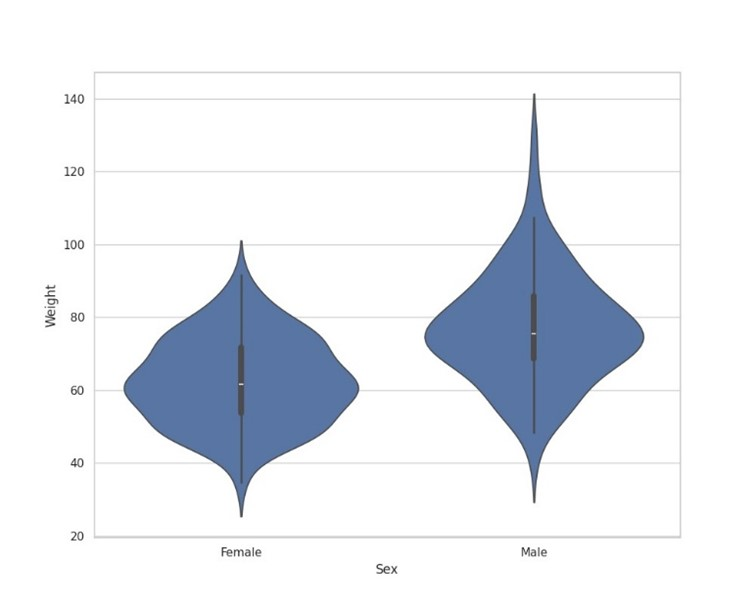
\includegraphics[width=0.5\textwidth]{violin_plot.jpg}
            \captionof{figure}{Weight plot between men and women}
            \label{fig:Violin_Plot}
        \end{center}
    \end{minipage}
    \item Pareto Chart:
    \begin{enumerate}
        \item Identify Major Issues: Highlights the most significant problems.
        \item Prioritize Actions: Focuses on key factors for improvement.
        \item Analyze Frequency: Shows which issues occur most frequently.
        \item Aid Decision-Making: Guides data-driven decisions
        \item Track Progress: Monitors changes in key issues over time.
    \end{enumerate}
    \begin{minipage}{\linewidth}
        \begin{center}
            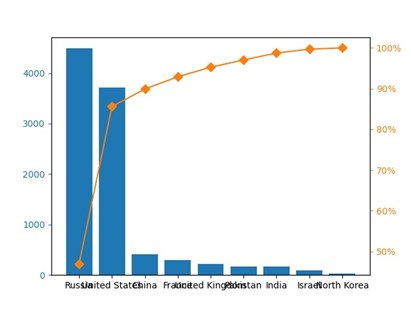
\includegraphics[width=0.5\textwidth]{pareto_chart.jpg}
            \captionof{figure}{Nuclear warhead in each country}
            \label{fig:Pareto_Chart}
        \end{center}
    \end{minipage}
    \item Coxcomb Chart(also known as Polar Area Chart):
    \begin{enumerate}
        \item Visualize Proportions: Display data in circular segments to show proportions and relationships among categories.
        \item Compare Multiple Variables: Compare various categories or time periods using radial sections.
        \item Highlight Trends: Illustrate patterns and trends in data over time or across different categories.
        \item Emphasize Differences: Show differences between categories or groups clearly through radial sections of varying sizes.
    \end{enumerate}
    \begin{minipage}{\linewidth}
        \begin{center}
            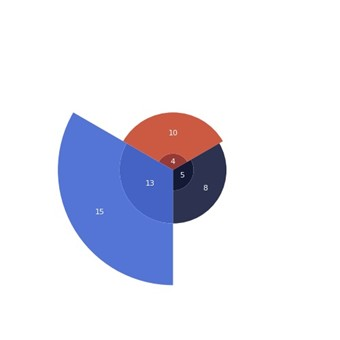
\includegraphics[width=0.5\textwidth]{Coxcomb chart.jpg}
            \captionof{figure}{Random data set}
            \label{fig:Coxcomb_chart}
        \end{center}
    \end{minipage}
    \item Waterfall plot
    \begin{enumerate}
        \item A waterfall plot is used to Show Sequential Changes: Illustrate how an initial value changes through various factors to reach a final value.
        \item Highlight Contributions: Display the impact of each factor on the overall change.
        \item Track Performance: Analyze financial metrics or performance over time.
        \item Reveal Trends: Identify trends and patterns in data.
    \end{enumerate} 
    \begin{minipage}{\linewidth}
        \begin{center}
            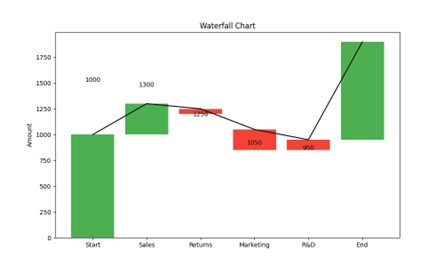
\includegraphics[width=0.5\textwidth]{Waterfall.jpg}
            \captionof{figure}{Random data set}
            \label{fig:Waterfall_plot}
        \end{center}
    \end{minipage}
\end{enumerate}

\section{Monalisa}
Download the image of Monalisa from here. Read the image using matplotlib example. Write a
piece of python code to shift the image along the X direction by $t_x$ pixels where $t_x$ is an integer
ranging from -10 to +10 (so, in total you need to do this for 20 values). While doing so, assign
a value of 0 to unoccupied pixels. For each shift, compute the correlation coefficient between the
original image and its shifted version. Make a plot of correlation coefficients across the shift values.
Also, generate a normalized histogram for the original image. You might need to refer to section
3.3 from this book. You are not allowed to use any inbuilt function for generating the histogram.
If you are using any other libraries, then please mention about them in the pdf.
\\
\\
\textbf{\Large{Refer to Monalisa.ipynb in Q8\_Monalisa Folder for the code and explanation. Run all the cells consecutively.}}
\\ \\ \\
\textbf{Libraries Used: } \\ 
\begin{enumerate}
    \item \textbf{\Large{matplotlib}}
    \item \textbf{\Large{numpy}}
\end{enumerate}
\end{document}